\chapter{Common-Source Amplifier}


\section{Objectives}
\begin{itemize}
    \item To measure the quiescent-point of a common-source amplifier
    \item To evaluate the small-signal amplification function of a common-source amplifier
\end{itemize}

\section{Materials}
\begin{itemize}
    \item Breadboard
    \item DC power supply
    \item Digital Multi-Meter
    \item Function Generator
    \item \hyperref[2N7000_1]{MOSFET (2N7000)}
    \item Oscilloscope
    \item Resistors
\end{itemize}

\section{Introduction}
    \subsection{Circuit Diagram}
    \begin{figure}[h]
        \centering
        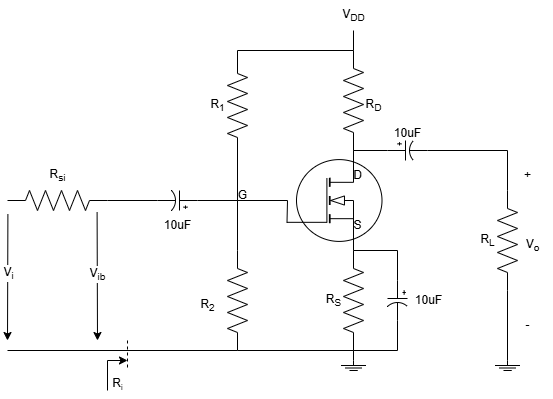
\includegraphics[width=0.65\linewidth]{Lab09/Lab9.drawio.png}
        \caption{Circuit Diagram}
        \label{l9f}
    \end{figure}
    \FloatBarrier

\section{Detailed Procedures}
    \subsection{Analyzation}
    \subsubsection{DC Analysis}
        \begin{figure}[h]
            \centering
            
\includegraphics[width=0.5\linewidth]{Lab09/L9DC.drawio.png}
            \caption{DC-Equivalent Circuit}
            \label{l9dc}
        \end{figure}
        \FloatBarrier
        \begin{equation*}
            \begin{cases}
                V_G=V_DD\frac{R_2}{R_1+R_2}\\
                V_{DS}=V_{DD}-I_DR_D-I_DR_S\\
                V_S=I_DR_S\\
                V_G-V_S>V_{TH}\\
                R_2<R_1\frac{2-V_{TH}}{V_{TH}-8}\\
            \end{cases}
        \end{equation*}
    \subsubsection{AC Analysis}
        \begin{figure}[h]
            \centering
            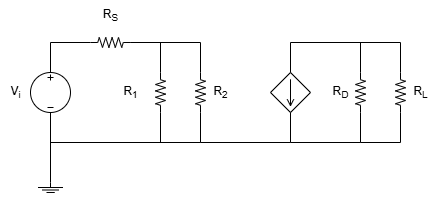
\includegraphics[width=0.5\linewidth]{Lab09/L9AC.drawio.png}
            \caption{AC-Equivalent Circuit}
            \label{l9ac}
        \end{figure}
        \FloatBarrier
        \begin{equation*}
            \begin{cases}
                A_v=-gm(R_D//R_L)\\
                R_i=R_1//R_2\\
                R_o=R_D//R_L\\
            \end{cases}
        \end{equation*}

        
    \subsection{Procedures}
    \subsubsection{DC Analysis}
    Shorted the $v_i$ to the ground and measured $I_DQ$ and $V_{DSQ}$ with digital multi-meter. For calibration, we adjusted $R_2$ to 68K.

    \subsubsection{AC Analysis: Voltage Gain}
    Let $v_i$ to be a sinusoidal signal (1000 Hz, 100mV peak), make sure the output voltage is not distorted with the help of the oscilloscope and record the plot. Now use the digital multi-meter to measure the rms value of $vi_b$ and $v_o$.\par
    Vary the input voltage amplitude to 80mV, 60mV, 40mV respectively.\\
    \begin{table}[h]
    \centering
    \begin{tabular}{|c|c|c|c|c|}
    \hline
    Vib & 0.0646 & 0.052 & 0.039 & 0.025 \\ \hline
    Vo  & 0.51   & 0.413 & 0.309 & 0.205 \\ \hline
    \end{tabular}
    \end{table}
    
    \subsubsection{AC Analysis: Input Resistance \& Output Resistance}
    \begin{itemize}
        \item Input Resistance: Let $v_i$ to be a 1000 Hz sinusoidal signal with the amplitude of 100 mV, make sure the output voltage is not distorted with the help of the oscilloscope.
        \item Output Resistance: Let $v_i$ to be a 1000 Hz sinusoidal signal with the amplitude of 100 mV, make sure the output voltage is not distorted with the help of the oscilloscope. Use the digital multi-meter to measure the rms values of output voltage vo when RL = 300k$\Omega$ and when RL = 1k$\Omega$ respectively.
    \end{itemize}
    Record data:\\
\begin{table}[h]
\centering
\resizebox{\columnwidth}{!}{%
\begin{tabular}{|cc|cc|}
\hline
\multicolumn{2}{|c|}{Rsi=4.7K,Ri=40.5K}    & \multicolumn{2}{c|}{Ro=199.9}                          \\ \hline
\multicolumn{1}{|c|}{Vi=0.072} & Vib=0.066 & \multicolumn{1}{c|}{RL=300K,Vo=0.522} & RL=1K,Vo=0.436 \\ \hline
\end{tabular}%
}
\end{table}
\FloatBarrier

    

\section{Conclusion}
This experiment presents us the common-source MOSFET amplifier. The experiment reinforces my understanding of the MOSFET circuit.\par
The common-source configuration effectively demonstrates voltage amplification, showcasing its ability to amplify small input signals into larger output signals. While the common-source amplifier offers high gain, it also exhibits nonlinearity at large input signal levels. During the experiment, we need to adjust input voltage to avoid the distortion.\par
In conclusion, the common-source MOSFET amplifier is a common building block in the small circuit design, it provides significant voltage amplification with high input impedance and moderate output impedance.